% Created by tikzDevice version 0.12.3.2 on 2022-02-07 12:37:59
% !TEX encoding = UTF-8 Unicode
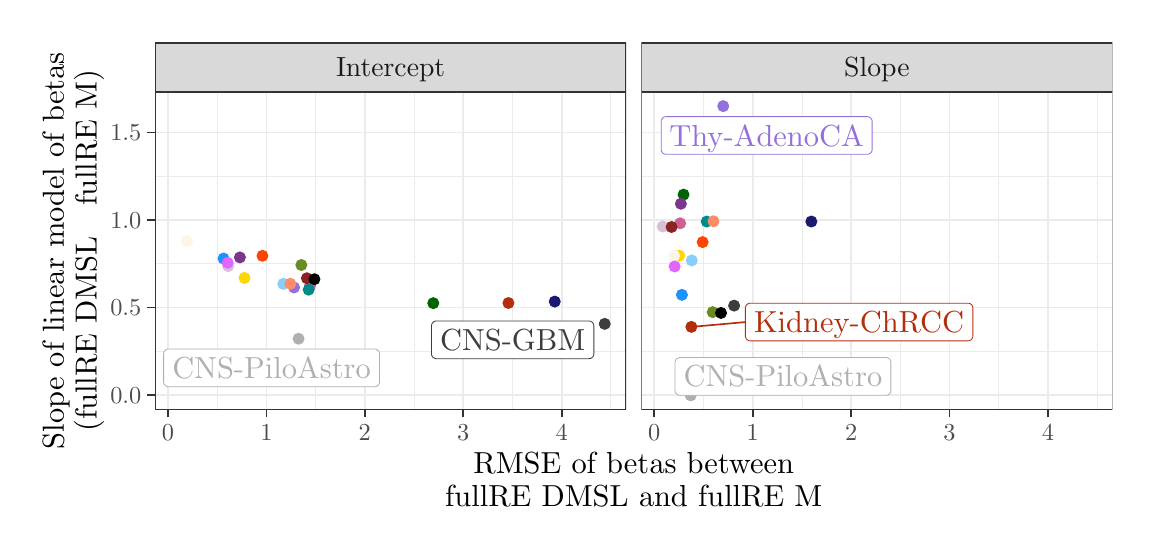
\begin{tikzpicture}[x=1pt,y=1pt]
\definecolor{fillColor}{RGB}{255,255,255}
\path[use as bounding box,fill=fillColor,fill opacity=0.00] (0,0) rectangle (397.48,180.67);
\begin{scope}
\path[clip] (  0.00,  0.00) rectangle (397.48,180.67);
\definecolor{drawColor}{RGB}{255,255,255}
\definecolor{fillColor}{RGB}{255,255,255}

\path[draw=drawColor,line width= 0.6pt,line join=round,line cap=round,fill=fillColor] (  0.00,  0.00) rectangle (397.48,180.68);
\end{scope}
\begin{scope}
\path[clip] ( 46.04, 42.57) rectangle (216.26,157.54);
\definecolor{fillColor}{RGB}{255,255,255}

\path[fill=fillColor] ( 46.04, 42.57) rectangle (216.26,157.54);
\definecolor{drawColor}{gray}{0.92}

\path[draw=drawColor,line width= 0.3pt,line join=round] ( 46.04, 63.75) --
	(216.26, 63.75);

\path[draw=drawColor,line width= 0.3pt,line join=round] ( 46.04, 95.36) --
	(216.26, 95.36);

\path[draw=drawColor,line width= 0.3pt,line join=round] ( 46.04,126.98) --
	(216.26,126.98);

\path[draw=drawColor,line width= 0.3pt,line join=round] ( 68.49, 42.57) --
	( 68.49,157.54);

\path[draw=drawColor,line width= 0.3pt,line join=round] (104.05, 42.57) --
	(104.05,157.54);

\path[draw=drawColor,line width= 0.3pt,line join=round] (139.62, 42.57) --
	(139.62,157.54);

\path[draw=drawColor,line width= 0.3pt,line join=round] (175.18, 42.57) --
	(175.18,157.54);

\path[draw=drawColor,line width= 0.3pt,line join=round] (210.74, 42.57) --
	(210.74,157.54);

\path[draw=drawColor,line width= 0.6pt,line join=round] ( 46.04, 47.94) --
	(216.26, 47.94);

\path[draw=drawColor,line width= 0.6pt,line join=round] ( 46.04, 79.55) --
	(216.26, 79.55);

\path[draw=drawColor,line width= 0.6pt,line join=round] ( 46.04,111.17) --
	(216.26,111.17);

\path[draw=drawColor,line width= 0.6pt,line join=round] ( 46.04,142.79) --
	(216.26,142.79);

\path[draw=drawColor,line width= 0.6pt,line join=round] ( 50.70, 42.57) --
	( 50.70,157.54);

\path[draw=drawColor,line width= 0.6pt,line join=round] ( 86.27, 42.57) --
	( 86.27,157.54);

\path[draw=drawColor,line width= 0.6pt,line join=round] (121.83, 42.57) --
	(121.83,157.54);

\path[draw=drawColor,line width= 0.6pt,line join=round] (157.40, 42.57) --
	(157.40,157.54);

\path[draw=drawColor,line width= 0.6pt,line join=round] (192.96, 42.57) --
	(192.96,157.54);
\definecolor{drawColor}{RGB}{255,215,0}
\definecolor{fillColor}{RGB}{255,215,0}

\path[draw=drawColor,line width= 0.4pt,line join=round,line cap=round,fill=fillColor] ( 78.35, 90.23) circle (  1.96);
\definecolor{drawColor}{RGB}{205,96,144}
\definecolor{fillColor}{RGB}{205,96,144}

\path[draw=drawColor,line width= 0.4pt,line join=round,line cap=round,fill=fillColor] (102.06, 87.52) circle (  1.96);
\definecolor{drawColor}{gray}{0.24}
\definecolor{fillColor}{gray}{0.24}

\path[draw=drawColor,line width= 0.4pt,line join=round,line cap=round,fill=fillColor] (208.52, 73.64) circle (  1.96);
\definecolor{drawColor}{RGB}{216,191,216}
\definecolor{fillColor}{RGB}{216,191,216}

\path[draw=drawColor,line width= 0.4pt,line join=round,line cap=round,fill=fillColor] ( 72.44, 94.52) circle (  1.96);
\definecolor{drawColor}{gray}{0.69}
\definecolor{fillColor}{gray}{0.69}

\path[draw=drawColor,line width= 0.4pt,line join=round,line cap=round,fill=fillColor] ( 97.88, 68.27) circle (  1.96);
\definecolor{drawColor}{RGB}{25,25,112}
\definecolor{fillColor}{RGB}{25,25,112}

\path[draw=drawColor,line width= 0.4pt,line join=round,line cap=round,fill=fillColor] (190.46, 81.69) circle (  1.96);
\definecolor{drawColor}{RGB}{30,144,255}
\definecolor{fillColor}{RGB}{30,144,255}

\path[draw=drawColor,line width= 0.4pt,line join=round,line cap=round,fill=fillColor] ( 70.78, 97.25) circle (  1.96);
\definecolor{drawColor}{RGB}{139,35,35}
\definecolor{fillColor}{RGB}{139,35,35}

\path[draw=drawColor,line width= 0.4pt,line join=round,line cap=round,fill=fillColor] (100.90, 90.13) circle (  1.96);
\definecolor{drawColor}{RGB}{179,47,11}
\definecolor{fillColor}{RGB}{179,47,11}

\path[draw=drawColor,line width= 0.4pt,line join=round,line cap=round,fill=fillColor] (173.72, 81.18) circle (  1.96);
\definecolor{drawColor}{RGB}{255,69,0}
\definecolor{fillColor}{RGB}{255,69,0}

\path[draw=drawColor,line width= 0.4pt,line join=round,line cap=round,fill=fillColor] ( 84.83, 98.23) circle (  1.96);
\definecolor{drawColor}{RGB}{0,100,0}
\definecolor{fillColor}{RGB}{0,100,0}

\path[draw=drawColor,line width= 0.4pt,line join=round,line cap=round,fill=fillColor] (146.56, 81.12) circle (  1.96);
\definecolor{drawColor}{RGB}{253,245,230}
\definecolor{fillColor}{RGB}{253,245,230}

\path[draw=drawColor,line width= 0.4pt,line join=round,line cap=round,fill=fillColor] ( 57.55,103.56) circle (  1.96);
\definecolor{drawColor}{RGB}{105,139,34}
\definecolor{fillColor}{RGB}{105,139,34}

\path[draw=drawColor,line width= 0.4pt,line join=round,line cap=round,fill=fillColor] ( 98.89, 94.91) circle (  1.96);
\definecolor{drawColor}{RGB}{0,139,139}
\definecolor{fillColor}{RGB}{0,139,139}

\path[draw=drawColor,line width= 0.4pt,line join=round,line cap=round,fill=fillColor] (101.54, 85.99) circle (  1.96);
\definecolor{drawColor}{RGB}{122,55,139}
\definecolor{fillColor}{RGB}{122,55,139}

\path[draw=drawColor,line width= 0.4pt,line join=round,line cap=round,fill=fillColor] ( 76.69, 97.66) circle (  1.96);
\definecolor{drawColor}{RGB}{224,102,255}
\definecolor{fillColor}{RGB}{224,102,255}

\path[draw=drawColor,line width= 0.4pt,line join=round,line cap=round,fill=fillColor] ( 72.26, 95.71) circle (  1.96);
\definecolor{drawColor}{RGB}{135,206,250}
\definecolor{fillColor}{RGB}{135,206,250}

\path[draw=drawColor,line width= 0.4pt,line join=round,line cap=round,fill=fillColor] ( 92.37, 88.09) circle (  1.96);
\definecolor{drawColor}{RGB}{0,0,0}
\definecolor{fillColor}{RGB}{0,0,0}

\path[draw=drawColor,line width= 0.4pt,line join=round,line cap=round,fill=fillColor] (103.61, 89.78) circle (  1.96);
\definecolor{drawColor}{RGB}{147,112,219}
\definecolor{fillColor}{RGB}{147,112,219}

\path[draw=drawColor,line width= 0.4pt,line join=round,line cap=round,fill=fillColor] ( 96.25, 86.78) circle (  1.96);
\definecolor{drawColor}{RGB}{255,140,105}
\definecolor{fillColor}{RGB}{255,140,105}

\path[draw=drawColor,line width= 0.4pt,line join=round,line cap=round,fill=fillColor] ( 94.91, 88.14) circle (  1.96);
\end{scope}
\begin{scope}
\path[clip] ( 46.04, 42.57) rectangle (216.26,157.54);
\definecolor{drawColor}{gray}{0.24}
\definecolor{fillColor}{RGB}{255,255,255}

\path[draw=drawColor,line width= 0.3pt,line join=round,line cap=round,fill=fillColor] (147.72, 61.05) --
	(202.79, 61.05) --
	(202.71, 61.05) --
	(203.00, 61.07) --
	(203.29, 61.12) --
	(203.56, 61.23) --
	(203.81, 61.37) --
	(204.04, 61.56) --
	(204.23, 61.77) --
	(204.39, 62.02) --
	(204.50, 62.29) --
	(204.57, 62.57) --
	(204.59, 62.86) --
	(204.59, 62.86) --
	(204.59, 72.87) --
	(204.59, 72.87) --
	(204.57, 73.16) --
	(204.50, 73.44) --
	(204.39, 73.71) --
	(204.23, 73.96) --
	(204.04, 74.18) --
	(203.81, 74.36) --
	(203.56, 74.50) --
	(203.29, 74.61) --
	(203.00, 74.67) --
	(202.79, 74.68) --
	(147.72, 74.68) --
	(147.94, 74.67) --
	(147.65, 74.68) --
	(147.36, 74.64) --
	(147.08, 74.56) --
	(146.82, 74.44) --
	(146.58, 74.27) --
	(146.37, 74.07) --
	(146.19, 73.84) --
	(146.06, 73.58) --
	(145.97, 73.30) --
	(145.92, 73.02) --
	(145.91, 72.87) --
	(145.91, 62.86) --
	(145.92, 63.01) --
	(145.92, 62.71) --
	(145.97, 62.43) --
	(146.06, 62.15) --
	(146.19, 61.89) --
	(146.37, 61.66) --
	(146.58, 61.46) --
	(146.82, 61.30) --
	(147.08, 61.17) --
	(147.36, 61.09) --
	(147.65, 61.05) --
	cycle;
\end{scope}
\begin{scope}
\path[clip] ( 46.04, 42.57) rectangle (216.26,157.54);
\definecolor{drawColor}{gray}{0.24}

\node[text=drawColor,anchor=base,inner sep=0pt, outer sep=0pt, scale=  1.10] at (175.25, 64.06) {CNS-GBM};
\definecolor{drawColor}{gray}{0.69}
\definecolor{fillColor}{RGB}{255,255,255}

\path[draw=drawColor,line width= 0.3pt,line join=round,line cap=round,fill=fillColor] ( 50.93, 50.92) --
	(125.32, 50.92) --
	(125.25, 50.92) --
	(125.54, 50.93) --
	(125.83, 50.99) --
	(126.10, 51.09) --
	(126.35, 51.24) --
	(126.57, 51.42) --
	(126.77, 51.64) --
	(126.92, 51.88) --
	(127.04, 52.15) --
	(127.11, 52.43) --
	(127.13, 52.72) --
	(127.13, 52.72) --
	(127.13, 62.74) --
	(127.13, 62.74) --
	(127.11, 63.03) --
	(127.04, 63.31) --
	(126.92, 63.58) --
	(126.77, 63.82) --
	(126.57, 64.04) --
	(126.35, 64.22) --
	(126.10, 64.37) --
	(125.83, 64.47) --
	(125.54, 64.53) --
	(125.32, 64.54) --
	( 50.93, 64.54) --
	( 51.14, 64.53) --
	( 50.85, 64.54) --
	( 50.56, 64.51) --
	( 50.29, 64.43) --
	( 50.02, 64.30) --
	( 49.78, 64.14) --
	( 49.57, 63.94) --
	( 49.40, 63.70) --
	( 49.26, 63.45) --
	( 49.17, 63.17) --
	( 49.13, 62.88) --
	( 49.12, 62.74) --
	( 49.12, 52.72) --
	( 49.13, 52.87) --
	( 49.13, 52.58) --
	( 49.17, 52.29) --
	( 49.26, 52.02) --
	( 49.40, 51.76) --
	( 49.57, 51.53) --
	( 49.78, 51.32) --
	( 50.02, 51.16) --
	( 50.29, 51.04) --
	( 50.56, 50.95) --
	( 50.85, 50.92) --
	cycle;
\end{scope}
\begin{scope}
\path[clip] ( 46.04, 42.57) rectangle (216.26,157.54);
\definecolor{drawColor}{gray}{0.69}

\node[text=drawColor,anchor=base,inner sep=0pt, outer sep=0pt, scale=  1.10] at ( 88.12, 53.93) {CNS-PiloAstro};
\definecolor{drawColor}{gray}{0.20}

\path[draw=drawColor,line width= 0.6pt,line join=round,line cap=round] ( 46.04, 42.57) rectangle (216.26,157.54);
\end{scope}
\begin{scope}
\path[clip] (221.76, 42.57) rectangle (391.98,157.54);
\definecolor{fillColor}{RGB}{255,255,255}

\path[fill=fillColor] (221.76, 42.57) rectangle (391.98,157.54);
\definecolor{drawColor}{gray}{0.92}

\path[draw=drawColor,line width= 0.3pt,line join=round] (221.76, 63.75) --
	(391.98, 63.75);

\path[draw=drawColor,line width= 0.3pt,line join=round] (221.76, 95.36) --
	(391.98, 95.36);

\path[draw=drawColor,line width= 0.3pt,line join=round] (221.76,126.98) --
	(391.98,126.98);

\path[draw=drawColor,line width= 0.3pt,line join=round] (244.21, 42.57) --
	(244.21,157.54);

\path[draw=drawColor,line width= 0.3pt,line join=round] (279.78, 42.57) --
	(279.78,157.54);

\path[draw=drawColor,line width= 0.3pt,line join=round] (315.34, 42.57) --
	(315.34,157.54);

\path[draw=drawColor,line width= 0.3pt,line join=round] (350.90, 42.57) --
	(350.90,157.54);

\path[draw=drawColor,line width= 0.3pt,line join=round] (386.47, 42.57) --
	(386.47,157.54);

\path[draw=drawColor,line width= 0.6pt,line join=round] (221.76, 47.94) --
	(391.98, 47.94);

\path[draw=drawColor,line width= 0.6pt,line join=round] (221.76, 79.55) --
	(391.98, 79.55);

\path[draw=drawColor,line width= 0.6pt,line join=round] (221.76,111.17) --
	(391.98,111.17);

\path[draw=drawColor,line width= 0.6pt,line join=round] (221.76,142.79) --
	(391.98,142.79);

\path[draw=drawColor,line width= 0.6pt,line join=round] (226.43, 42.57) --
	(226.43,157.54);

\path[draw=drawColor,line width= 0.6pt,line join=round] (261.99, 42.57) --
	(261.99,157.54);

\path[draw=drawColor,line width= 0.6pt,line join=round] (297.56, 42.57) --
	(297.56,157.54);

\path[draw=drawColor,line width= 0.6pt,line join=round] (333.12, 42.57) --
	(333.12,157.54);

\path[draw=drawColor,line width= 0.6pt,line join=round] (368.69, 42.57) --
	(368.69,157.54);
\definecolor{drawColor}{RGB}{255,215,0}
\definecolor{fillColor}{RGB}{255,215,0}

\path[draw=drawColor,line width= 0.4pt,line join=round,line cap=round,fill=fillColor] (235.45, 98.28) circle (  1.96);
\definecolor{drawColor}{RGB}{205,96,144}
\definecolor{fillColor}{RGB}{205,96,144}

\path[draw=drawColor,line width= 0.4pt,line join=round,line cap=round,fill=fillColor] (235.76,109.98) circle (  1.96);
\definecolor{drawColor}{gray}{0.24}
\definecolor{fillColor}{gray}{0.24}

\path[draw=drawColor,line width= 0.4pt,line join=round,line cap=round,fill=fillColor] (255.27, 80.23) circle (  1.96);
\definecolor{drawColor}{RGB}{216,191,216}
\definecolor{fillColor}{RGB}{216,191,216}

\path[draw=drawColor,line width= 0.4pt,line join=round,line cap=round,fill=fillColor] (229.50,108.81) circle (  1.96);
\definecolor{drawColor}{gray}{0.69}
\definecolor{fillColor}{gray}{0.69}

\path[draw=drawColor,line width= 0.4pt,line join=round,line cap=round,fill=fillColor] (239.60, 47.79) circle (  1.96);
\definecolor{drawColor}{RGB}{25,25,112}
\definecolor{fillColor}{RGB}{25,25,112}

\path[draw=drawColor,line width= 0.4pt,line join=round,line cap=round,fill=fillColor] (283.18,110.62) circle (  1.96);
\definecolor{drawColor}{RGB}{30,144,255}
\definecolor{fillColor}{RGB}{30,144,255}

\path[draw=drawColor,line width= 0.4pt,line join=round,line cap=round,fill=fillColor] (236.41, 84.13) circle (  1.96);
\definecolor{drawColor}{RGB}{139,35,35}
\definecolor{fillColor}{RGB}{139,35,35}

\path[draw=drawColor,line width= 0.4pt,line join=round,line cap=round,fill=fillColor] (232.68,108.65) circle (  1.96);
\definecolor{drawColor}{RGB}{179,47,11}
\definecolor{fillColor}{RGB}{179,47,11}

\path[draw=drawColor,line width= 0.4pt,line join=round,line cap=round,fill=fillColor] (239.82, 72.55) circle (  1.96);
\definecolor{drawColor}{RGB}{255,69,0}
\definecolor{fillColor}{RGB}{255,69,0}

\path[draw=drawColor,line width= 0.4pt,line join=round,line cap=round,fill=fillColor] (243.90,103.18) circle (  1.96);
\definecolor{drawColor}{RGB}{0,100,0}
\definecolor{fillColor}{RGB}{0,100,0}

\path[draw=drawColor,line width= 0.4pt,line join=round,line cap=round,fill=fillColor] (237.00,120.34) circle (  1.96);
\definecolor{drawColor}{RGB}{253,245,230}
\definecolor{fillColor}{RGB}{253,245,230}

\path[draw=drawColor,line width= 0.4pt,line join=round,line cap=round,fill=fillColor] (233.62, 98.21) circle (  1.96);
\definecolor{drawColor}{RGB}{105,139,34}
\definecolor{fillColor}{RGB}{105,139,34}

\path[draw=drawColor,line width= 0.4pt,line join=round,line cap=round,fill=fillColor] (247.52, 77.89) circle (  1.96);
\definecolor{drawColor}{RGB}{0,139,139}
\definecolor{fillColor}{RGB}{0,139,139}

\path[draw=drawColor,line width= 0.4pt,line join=round,line cap=round,fill=fillColor] (245.37,110.61) circle (  1.96);
\definecolor{drawColor}{RGB}{122,55,139}
\definecolor{fillColor}{RGB}{122,55,139}

\path[draw=drawColor,line width= 0.4pt,line join=round,line cap=round,fill=fillColor] (236.03,117.04) circle (  1.96);
\definecolor{drawColor}{RGB}{224,102,255}
\definecolor{fillColor}{RGB}{224,102,255}

\path[draw=drawColor,line width= 0.4pt,line join=round,line cap=round,fill=fillColor] (233.78, 94.38) circle (  1.96);
\definecolor{drawColor}{RGB}{135,206,250}
\definecolor{fillColor}{RGB}{135,206,250}

\path[draw=drawColor,line width= 0.4pt,line join=round,line cap=round,fill=fillColor] (239.97, 96.56) circle (  1.96);
\definecolor{drawColor}{RGB}{0,0,0}
\definecolor{fillColor}{RGB}{0,0,0}

\path[draw=drawColor,line width= 0.4pt,line join=round,line cap=round,fill=fillColor] (250.54, 77.59) circle (  1.96);
\definecolor{drawColor}{RGB}{147,112,219}
\definecolor{fillColor}{RGB}{147,112,219}

\path[draw=drawColor,line width= 0.4pt,line join=round,line cap=round,fill=fillColor] (251.33,152.32) circle (  1.96);
\definecolor{drawColor}{RGB}{255,140,105}
\definecolor{fillColor}{RGB}{255,140,105}

\path[draw=drawColor,line width= 0.4pt,line join=round,line cap=round,fill=fillColor] (247.82,110.72) circle (  1.96);
\end{scope}
\begin{scope}
\path[clip] (221.76, 42.57) rectangle (391.98,157.54);
\definecolor{drawColor}{RGB}{179,47,11}

\path[draw=drawColor,line width= 0.6pt,line join=round,line cap=round] (259.34, 74.28) -- (240.98, 72.65);
\definecolor{drawColor}{gray}{0.69}
\definecolor{fillColor}{RGB}{255,255,255}

\path[draw=drawColor,line width= 0.3pt,line join=round,line cap=round,fill=fillColor] (235.72, 47.84) --
	(310.12, 47.84) --
	(310.04, 47.84) --
	(310.34, 47.85) --
	(310.62, 47.91) --
	(310.89, 48.01) --
	(311.14, 48.16) --
	(311.37, 48.34) --
	(311.56, 48.56) --
	(311.72, 48.80) --
	(311.83, 49.07) --
	(311.90, 49.35) --
	(311.92, 49.64) --
	(311.92, 49.64) --
	(311.92, 59.65) --
	(311.92, 59.65) --
	(311.90, 59.94) --
	(311.83, 60.23) --
	(311.72, 60.49) --
	(311.56, 60.74) --
	(311.37, 60.96) --
	(311.14, 61.14) --
	(310.89, 61.29) --
	(310.62, 61.39) --
	(310.34, 61.45) --
	(310.12, 61.46) --
	(235.72, 61.46) --
	(235.94, 61.45) --
	(235.65, 61.46) --
	(235.36, 61.42) --
	(235.08, 61.34) --
	(234.82, 61.22) --
	(234.58, 61.05) --
	(234.37, 60.85) --
	(234.19, 60.62) --
	(234.06, 60.36) --
	(233.97, 60.09) --
	(233.92, 59.80) --
	(233.91, 59.65) --
	(233.91, 49.64) --
	(233.92, 49.79) --
	(233.92, 49.50) --
	(233.97, 49.21) --
	(234.06, 48.93) --
	(234.19, 48.68) --
	(234.37, 48.44) --
	(234.58, 48.24) --
	(234.82, 48.08) --
	(235.08, 47.95) --
	(235.36, 47.87) --
	(235.65, 47.84) --
	cycle;
\end{scope}
\begin{scope}
\path[clip] (221.76, 42.57) rectangle (391.98,157.54);
\definecolor{drawColor}{gray}{0.69}

\node[text=drawColor,anchor=base,inner sep=0pt, outer sep=0pt, scale=  1.10] at (272.92, 50.85) {CNS-PiloAstro};
\definecolor{drawColor}{RGB}{179,47,11}
\definecolor{fillColor}{RGB}{255,255,255}

\path[draw=drawColor,line width= 0.3pt,line join=round,line cap=round,fill=fillColor] (261.15, 67.48) --
	(339.75, 67.48) --
	(339.67, 67.49) --
	(339.96, 67.50) --
	(340.25, 67.55) --
	(340.52, 67.66) --
	(340.77, 67.80) --
	(341.00, 67.99) --
	(341.19, 68.20) --
	(341.35, 68.45) --
	(341.46, 68.72) --
	(341.53, 69.00) --
	(341.55, 69.29) --
	(341.55, 69.29) --
	(341.55, 79.30) --
	(341.55, 79.30) --
	(341.53, 79.59) --
	(341.46, 79.87) --
	(341.35, 80.14) --
	(341.19, 80.39) --
	(341.00, 80.61) --
	(340.77, 80.79) --
	(340.52, 80.94) --
	(340.25, 81.04) --
	(339.96, 81.10) --
	(339.75, 81.11) --
	(261.15, 81.11) --
	(261.37, 81.10) --
	(261.08, 81.11) --
	(260.79, 81.07) --
	(260.51, 80.99) --
	(260.25, 80.87) --
	(260.01, 80.70) --
	(259.80, 80.50) --
	(259.62, 80.27) --
	(259.49, 80.01) --
	(259.40, 79.74) --
	(259.35, 79.45) --
	(259.34, 79.30) --
	(259.34, 69.29) --
	(259.35, 69.44) --
	(259.35, 69.14) --
	(259.40, 68.86) --
	(259.49, 68.58) --
	(259.62, 68.32) --
	(259.80, 68.09) --
	(260.01, 67.89) --
	(260.25, 67.73) --
	(260.51, 67.60) --
	(260.79, 67.52) --
	(261.08, 67.49) --
	cycle;
\end{scope}
\begin{scope}
\path[clip] (221.76, 42.57) rectangle (391.98,157.54);
\definecolor{drawColor}{RGB}{179,47,11}

\node[text=drawColor,anchor=base,inner sep=0pt, outer sep=0pt, scale=  1.10] at (300.45, 70.49) {Kidney-ChRCC};
\definecolor{drawColor}{RGB}{147,112,219}
\definecolor{fillColor}{RGB}{255,255,255}

\path[draw=drawColor,line width= 0.3pt,line join=round,line cap=round,fill=fillColor] (230.73,134.90) --
	(303.35,134.90) --
	(303.27,134.90) --
	(303.56,134.91) --
	(303.85,134.97) --
	(304.12,135.07) --
	(304.37,135.22) --
	(304.60,135.40) --
	(304.79,135.62) --
	(304.95,135.87) --
	(305.06,136.13) --
	(305.13,136.42) --
	(305.15,136.71) --
	(305.15,136.71) --
	(305.15,146.72) --
	(305.15,146.72) --
	(305.13,147.01) --
	(305.06,147.29) --
	(304.95,147.56) --
	(304.79,147.80) --
	(304.60,148.02) --
	(304.37,148.20) --
	(304.12,148.35) --
	(303.85,148.45) --
	(303.56,148.51) --
	(303.35,148.52) --
	(230.73,148.52) --
	(230.94,148.51) --
	(230.65,148.52) --
	(230.37,148.49) --
	(230.09,148.41) --
	(229.82,148.28) --
	(229.58,148.12) --
	(229.37,147.92) --
	(229.20,147.68) --
	(229.06,147.43) --
	(228.97,147.15) --
	(228.93,146.86) --
	(228.92,146.72) --
	(228.92,136.71) --
	(228.93,136.85) --
	(228.93,136.56) --
	(228.97,136.27) --
	(229.06,136.00) --
	(229.20,135.74) --
	(229.37,135.51) --
	(229.58,135.31) --
	(229.82,135.14) --
	(230.09,135.02) --
	(230.37,134.93) --
	(230.65,134.90) --
	cycle;
\end{scope}
\begin{scope}
\path[clip] (221.76, 42.57) rectangle (391.98,157.54);
\definecolor{drawColor}{RGB}{147,112,219}

\node[text=drawColor,anchor=base,inner sep=0pt, outer sep=0pt, scale=  1.10] at (267.04,137.91) {Thy-AdenoCA};
\definecolor{drawColor}{gray}{0.20}

\path[draw=drawColor,line width= 0.6pt,line join=round,line cap=round] (221.76, 42.57) rectangle (391.98,157.54);
\end{scope}
\begin{scope}
\path[clip] ( 46.04,157.54) rectangle (216.26,175.17);
\definecolor{drawColor}{gray}{0.20}
\definecolor{fillColor}{gray}{0.85}

\path[draw=drawColor,line width= 0.6pt,line join=round,line cap=round,fill=fillColor] ( 46.04,157.54) rectangle (216.26,175.17);
\definecolor{drawColor}{gray}{0.10}

\node[text=drawColor,anchor=base,inner sep=0pt, outer sep=0pt, scale=  1.00] at (131.15,162.92) {Intercept};
\end{scope}
\begin{scope}
\path[clip] (221.76,157.54) rectangle (391.98,175.17);
\definecolor{drawColor}{gray}{0.20}
\definecolor{fillColor}{gray}{0.85}

\path[draw=drawColor,line width= 0.6pt,line join=round,line cap=round,fill=fillColor] (221.76,157.54) rectangle (391.98,175.17);
\definecolor{drawColor}{gray}{0.10}

\node[text=drawColor,anchor=base,inner sep=0pt, outer sep=0pt, scale=  1.00] at (306.87,162.92) {Slope};
\end{scope}
\begin{scope}
\path[clip] (  0.00,  0.00) rectangle (397.48,180.67);
\definecolor{drawColor}{gray}{0.20}

\path[draw=drawColor,line width= 0.6pt,line join=round] ( 50.70, 39.82) --
	( 50.70, 42.57);

\path[draw=drawColor,line width= 0.6pt,line join=round] ( 86.27, 39.82) --
	( 86.27, 42.57);

\path[draw=drawColor,line width= 0.6pt,line join=round] (121.83, 39.82) --
	(121.83, 42.57);

\path[draw=drawColor,line width= 0.6pt,line join=round] (157.40, 39.82) --
	(157.40, 42.57);

\path[draw=drawColor,line width= 0.6pt,line join=round] (192.96, 39.82) --
	(192.96, 42.57);
\end{scope}
\begin{scope}
\path[clip] (  0.00,  0.00) rectangle (397.48,180.67);
\definecolor{drawColor}{gray}{0.30}

\node[text=drawColor,anchor=base,inner sep=0pt, outer sep=0pt, scale=  0.88] at ( 50.70, 31.56) {0};

\node[text=drawColor,anchor=base,inner sep=0pt, outer sep=0pt, scale=  0.88] at ( 86.27, 31.56) {1};

\node[text=drawColor,anchor=base,inner sep=0pt, outer sep=0pt, scale=  0.88] at (121.83, 31.56) {2};

\node[text=drawColor,anchor=base,inner sep=0pt, outer sep=0pt, scale=  0.88] at (157.40, 31.56) {3};

\node[text=drawColor,anchor=base,inner sep=0pt, outer sep=0pt, scale=  0.88] at (192.96, 31.56) {4};
\end{scope}
\begin{scope}
\path[clip] (  0.00,  0.00) rectangle (397.48,180.67);
\definecolor{drawColor}{gray}{0.20}

\path[draw=drawColor,line width= 0.6pt,line join=round] (226.43, 39.82) --
	(226.43, 42.57);

\path[draw=drawColor,line width= 0.6pt,line join=round] (261.99, 39.82) --
	(261.99, 42.57);

\path[draw=drawColor,line width= 0.6pt,line join=round] (297.56, 39.82) --
	(297.56, 42.57);

\path[draw=drawColor,line width= 0.6pt,line join=round] (333.12, 39.82) --
	(333.12, 42.57);

\path[draw=drawColor,line width= 0.6pt,line join=round] (368.69, 39.82) --
	(368.69, 42.57);
\end{scope}
\begin{scope}
\path[clip] (  0.00,  0.00) rectangle (397.48,180.67);
\definecolor{drawColor}{gray}{0.30}

\node[text=drawColor,anchor=base,inner sep=0pt, outer sep=0pt, scale=  0.88] at (226.43, 31.56) {0};

\node[text=drawColor,anchor=base,inner sep=0pt, outer sep=0pt, scale=  0.88] at (261.99, 31.56) {1};

\node[text=drawColor,anchor=base,inner sep=0pt, outer sep=0pt, scale=  0.88] at (297.56, 31.56) {2};

\node[text=drawColor,anchor=base,inner sep=0pt, outer sep=0pt, scale=  0.88] at (333.12, 31.56) {3};

\node[text=drawColor,anchor=base,inner sep=0pt, outer sep=0pt, scale=  0.88] at (368.69, 31.56) {4};
\end{scope}
\begin{scope}
\path[clip] (  0.00,  0.00) rectangle (397.48,180.67);
\definecolor{drawColor}{gray}{0.30}

\node[text=drawColor,anchor=base east,inner sep=0pt, outer sep=0pt, scale=  0.88] at ( 41.09, 44.91) {0.0};

\node[text=drawColor,anchor=base east,inner sep=0pt, outer sep=0pt, scale=  0.88] at ( 41.09, 76.52) {0.5};

\node[text=drawColor,anchor=base east,inner sep=0pt, outer sep=0pt, scale=  0.88] at ( 41.09,108.14) {1.0};

\node[text=drawColor,anchor=base east,inner sep=0pt, outer sep=0pt, scale=  0.88] at ( 41.09,139.76) {1.5};
\end{scope}
\begin{scope}
\path[clip] (  0.00,  0.00) rectangle (397.48,180.67);
\definecolor{drawColor}{gray}{0.20}

\path[draw=drawColor,line width= 0.6pt,line join=round] ( 43.29, 47.94) --
	( 46.04, 47.94);

\path[draw=drawColor,line width= 0.6pt,line join=round] ( 43.29, 79.55) --
	( 46.04, 79.55);

\path[draw=drawColor,line width= 0.6pt,line join=round] ( 43.29,111.17) --
	( 46.04,111.17);

\path[draw=drawColor,line width= 0.6pt,line join=round] ( 43.29,142.79) --
	( 46.04,142.79);
\end{scope}
\begin{scope}
\path[clip] (  0.00,  0.00) rectangle (397.48,180.67);
\definecolor{drawColor}{RGB}{0,0,0}

\node[text=drawColor,anchor=base,inner sep=0pt, outer sep=0pt, scale=  1.10] at (219.01, 19.52) {RMSE of betas between};

\node[text=drawColor,anchor=base,inner sep=0pt, outer sep=0pt, scale=  1.10] at (219.01,  7.64) {fullRE DMSL and fullRE M};
\end{scope}
\begin{scope}
\path[clip] (  0.00,  0.00) rectangle (397.48,180.67);
\definecolor{drawColor}{RGB}{0,0,0}

\node[text=drawColor,rotate= 90.00,anchor=base,inner sep=0pt, outer sep=0pt, scale=  1.10] at ( 13.08,100.05) {Slope of linear model of betas};

\node[text=drawColor,rotate= 90.00,anchor=base,inner sep=0pt, outer sep=0pt, scale=  1.10] at ( 24.96,100.05) {(fullRE DMSL ~ fullRE M)};
\end{scope}
\end{tikzpicture}
